\documentclass[11pt]{article}
\usepackage{fullpage}
\usepackage{graphics,epsfig,color}
\usepackage{wrapfig}

\usepackage{times}
\usepackage{setspace}
\usepackage{amsmath,amsthm,amssymb}
%\usepackage[ruled,vlined,linesnumbered]{algorithm2e}
\usepackage{qtree}
\usepackage{subfigure}
\usepackage{url}
\usepackage{tikz}


%for code from latexdraw
%\usepackage[usenames,dvipsnames]{pstricks}
%\usepackage{epsfig}
%\usepackage{pst-grad} % For gradients
%\usepackage{pst-plot} % For axes


\newtheorem{theorem}{Theorem}[section]
%\newtheorem{proposition}{Proposition}[theorem]
\newtheorem{corollary}{Corollary}[section]
\newtheorem{lemma}{Lemma}[section]
%\newtheorem{claim}{Claim}[section]
\newtheorem{problem}{Problem}
%\newtheorem{conjecture}{Conjecture}[section]
\newtheorem{definition}{Definition}[section]
\newtheorem{observation}{Observation}[section]
\newtheorem{example}{Example}[section]
\newtheorem{openproblem}{Open Problem}[section]
\newtheorem{fact}{Fact}[section]
%\newcommand{\qedsymb}{\hfill{\rule{2mm}{2mm}}}

\newcommand{\qedsymb}{\hfill{\rule{2mm}{2mm}}}
\newenvironment{proofsketch}{\begin{trivlist}
\item[\hspace{\labelsep}{\noindent Proof Sketch: }]
}{\qedsymb\end{trivlist}}



%the following few lines until usepackage{algorithm2e} is to avoid the
%conflicts of algorithm2e with other packages.
\makeatletter
\newif\if@restonecol
\makeatother
\let\algorithm\relax
\let\endalgorithm\relax
%\usepackage[ruled,vlined,linesnumbered]{algorithm2e}
\usepackage[ruled,vlined,linesnumbered]{algorithm2e}


%\newenvironment{proof}{\begin{trivlist}
%\item[\hspace{\labelsep}{\bf\noindent Proof: }]}{\qedsymb\end{trivlist}}
%\newcommand{\qed}{\hfill\rule{2mm}{2mm}}

\newcommand{\remove}[1]{}



%--------------------------------


\begin{document}

\begin{center}
  {\LARGE CSCD501 Homework3}

\bigskip 

{\Large Will Czifro}

\end{center}

\bigskip 

\begin{problem}[20 points]
\label{prob:1}
 In class, we analyzed that the false matching probability of the Karp-Rabin algorithm for
a binary sequence is no more than $\pi(nm)/\pi(I)$, where $n$ is the sequence size, $m$ is the pattern size, and $\pi(x)$ is
the number of positive prime numbers that are no larger than $x$. Now consider the case where the sequence and
the pattern are drawn from an alphabet of size $\sigma$. Can you analyze the false matching probably of the Karp-Rabin
algorithm for this general setting ? According to the result from your analysis, what is the false matching probability
if we set $I = n^2m$ ?
\end{problem}


%---------------------------------------

\begin{problem}[25 points]
\label{prob:2}
 Draw the automata for the pattern alabama for pattern matching. You can assume the
alphabet where the sequence is drawn from is $\Sigma = {a, b, l, m}$. Explain which state is the "starting state" and which
state is the "acceptance state".
\end{problem}



%---------------------------------------

\begin{problem}[30 points]
\label{prob:3}
Consider a sequence $S$ of size $n$ which is drawn from an alphabet $\Sigma = {0, 1,..., σ − 1}$. The
\textbf{0-order empirical entropy} of the sequence S is defined as

$$
H_0(S) = \sum_{i=0}^{\sigma-1} \frac{n_i}{n} log_2 \frac{n}{n_i}
$$

where $n_i$ is the number of copies of the character $i$ in $S$. Then, the \textbf{0-order empirical entropy compressed size} of $S$
is defined as $nH_0(S)$. \footnote{Clearly, the definition of the 0-order empirical entropy is also valid for a bit sequence where the alphabet is just ${0, 1}$.} %\newline

Now suppose you are given such a sequence $S$ and you create a wavelet tree for $S$. It’s easy to see that the wavelet
tree will have exactly $\sigma-1$ internal nodes, because the wavelet tree is a full binary tree \footnote{A full binary tree is a binary tree where all non-leaf nodes have exactly two children.}. Recall that each internal
node in the wavelet tree has a bit sequence. Let’s name these $(\sigma-1)$ bit sequences as $B_0, B_1,...,B_{\sigma-2}$.

Prove the following amazing claim is true, regardless of the shape of the wavelet tree:

$$
nH_0(S) = \sum_{i=0}^{\sigma-2}|B_i|H_0(B_i)
$$

where $|B_i|$ is the number of bits in the bit sequence $B_i$, $for$ $i = 0, 1,..., \sigma-1$. (This claim says a 0-order entropy
compression of all the bit sequences automatically gives a 0-order entropy compression of the original sequence $S$.)
Hint: use the inductive proof idea and play with the definition of the entropy. Note that any subtree of the wavelet
tree is also a wavelet tree for a subsequence (not of neighboring letters in the original sequence of course).

\end{problem}




\begin{problem}[25 points]
\label{prob:4}
Suffix array is another elegant data structure for sequence indexing and pattern matching.
The suffix array $SA[0, 1,...,n-1]$ of a sequence $S[0,1,...,n-1]$ is a permutation of ${0, 1,...,n-1}$, such that
all the suffixes of $S: S[SA[0],...,n-1]$, $S[SA[1],...,n-1]$,...,$S[SA[n-1],...,n-1]$ are in the ascending
lexicographic order.

Now suppose you are given the $BWT$ of the sequence $S$ as well as the location of the last character $S[n-1] =' \$'$
in the $BWT$, can you use the $BWT$ to construct the suffix array of $S$ ? Explain your idea and give the pseudocode.
(Hint: use idea for reversing the $BWT$.)

\end{problem}


%---------------------------------------

\bigskip
\noindent{\bf Solution for Problem~\ref{prob:1}.}

\begin{proof}

The probability of a false positive with a base $\sigma$ character set is:

$$
P_r(\epsilon) \leq \frac{2.53log_2(\sigma)}{n}
$$

To understand why this is true, we need to evaluate the following in terms of base 2:

$$
\prod_{r \in R} |H(P) - H(T_r)| \leq \sigma^{mn}
$$

We know that when $\sigma = 2$, that for $2^{mn}$ there are at most $\pi(mn)$ prime divisors.
However, for all other $\sigma \geq 2$, since a character set of base 1 is impractical, we
need to determine what $\sigma$ is equal to in terms of 2. A simple way to do this is to change
base by doing $a = b ^ {log_b(a)}$. So, $\sigma = 2^{log_2(\sigma)}$. Since in the above equation
it is $\sigma^{mn}$, then it is $2^{mnlog_2(\sigma)}$ and there are at most $\pi(mnlog_2(\sigma))$.
We now can say the following:

\begin{align*}
P_r(\epsilon) &= \frac{ \pi\big(mnlog_2(\sigma)\big) }{ \pi(I) } \\
              &= \frac{ \pi\big(mnlog_2(\sigma)\big) }{ \pi(mn^2) } \\
              &\leq \frac{ 1.26\frac{ mnlog_2(\sigma) }{ ln\big(mnlog_2(\sigma)\big) } }{ \frac{ mn^2 }{ ln(mn^2) } } \\
              &= 1.26 \frac{ mnlog_2(\sigma)ln(mn^2) }{ mn^2ln\big(mnlog_2(\sigma)\big) } \\
              &= 1.26 \frac{ log_2(\sigma) }{ n } \cdot \frac{ ln(m) + 2ln(n) }{ ln(m) + ln(n) + ln \big( log_2(\sigma) \big) } \\
              &\leq 1.26 \frac{ log_2(\sigma) }{ n } \cdot \frac{ 2ln(m) + 2ln(n) + 2ln\big(log_2(\sigma)\big) }{ ln(m) + ln(n) + ln\big(log_2(\sigma)\big) } \\
              &= 1.26 \frac{ log_2(\sigma) }{ n } \cdot \frac{ 2\Big(ln(m) + ln(n) + ln\big(log_2(\sigma)\big)\Big) }{ ln(m) + ln(n) + ln\big(log_2(\sigma)\big) } \\
              &= 1.26 \frac{ log_2(\sigma) }{ n } \cdot 2 \\
              &\leq \frac{ 2.53log_2(\sigma) }{ n }
\end{align*}

\end{proof}

%---------------------------------------

\bigskip
\noindent{\bf Solution for Problem~\ref{prob:2}.}

\begin{center}
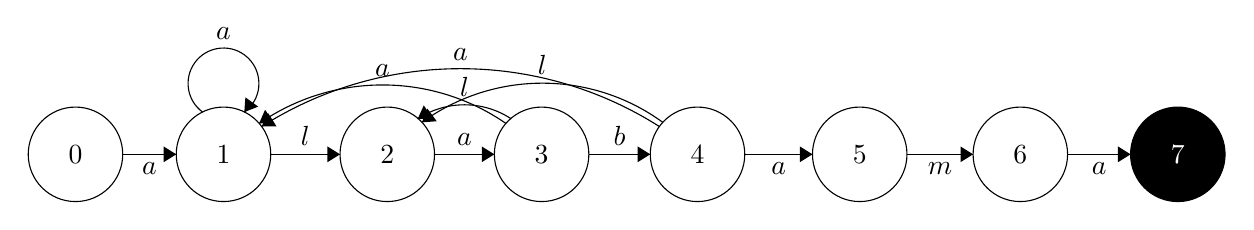
\begin{tikzpicture}[scale=0.2]
\tikzstyle{every node}+=[inner sep=0pt]
\draw [black] (5.2,-29.1) circle (3);
\draw (5.2,-29.1) node {$0$};
\draw [black] (14.6,-29.1) circle (3);
\draw (14.6,-29.1) node {$1$};
\draw [black] (25,-29.1) circle (3);
\draw (25,-29.1) node {$2$};
\draw [black] (34.8,-29.1) circle (3);
\draw (34.8,-29.1) node {$3$};
\draw [black] (44.7,-29.1) circle (3);
\draw (44.7,-29.1) node {$4$};
\draw [black] (55,-29.1) circle (3);
\draw (55,-29.1) node {$5$};
\draw [black] (65.2,-29.1) circle (3);
\draw (65.2,-29.1) node {$6$};
\draw [black,fill=black] (75.2,-29.1) circle (3);
\draw (75.2,-29.1) node {\color{white}$7$};
\draw [black] (8.2,-29.1) -- (11.6,-29.1);
\fill [black] (11.6,-29.1) -- (10.8,-28.6) -- (10.8,-29.6);
\draw (9.9,-29.6) node [below] {$a$};
\draw [black] (17.6,-29.1) -- (22,-29.1);
\fill [black] (22,-29.1) -- (21.2,-28.6) -- (21.2,-29.6);
\draw (19.8,-28.6) node [above] {$l$};
\draw [black] (28,-29.1) -- (31.8,-29.1);
\fill [black] (31.8,-29.1) -- (31,-28.6) -- (31,-29.6);
\draw (29.9,-28.6) node [above] {$a$};
\draw [black] (37.8,-29.1) -- (41.7,-29.1);
\fill [black] (41.7,-29.1) -- (40.9,-28.6) -- (40.9,-29.6);
\draw (39.75,-28.6) node [above] {$b$};
\draw [black] (47.7,-29.1) -- (52,-29.1);
\fill [black] (52,-29.1) -- (51.2,-28.6) -- (51.2,-29.6);
\draw (49.85,-29.6) node [below] {$a$};
\draw [black] (58,-29.1) -- (62.2,-29.1);
\fill [black] (62.2,-29.1) -- (61.4,-28.6) -- (61.4,-29.6);
\draw (60.1,-29.6) node [below] {$m$};
\draw [black] (68.2,-29.1) -- (72.2,-29.1);
\fill [black] (72.2,-29.1) -- (71.4,-28.6) -- (71.4,-29.6);
\draw (70.2,-29.6) node [below] {$a$};
\draw [black] (26.925,-26.85) arc (123.50376:56.49624:5.389);
\fill [black] (26.93,-26.85) -- (27.87,-26.83) -- (27.32,-25.99);
\draw (29.9,-25.45) node [above] {$l$};
\draw [black] (13.277,-26.42) arc (234:-54:2.25);
\draw (14.6,-21.85) node [above] {$a$};
\fill [black] (15.92,-26.42) -- (16.8,-26.07) -- (15.99,-25.48);
\draw [black] (16.863,-27.14) arc (124.66146:55.33854:13.78);
\fill [black] (16.86,-27.14) -- (17.81,-27.1) -- (17.24,-26.27);
\draw (24.7,-24.19) node [above] {$a$};
\draw [black] (17.023,-27.334) arc (122.43631:57.56369:23.542);
\fill [black] (17.02,-27.33) -- (17.97,-27.33) -- (17.43,-26.48);
\draw (29.65,-23.16) node [above] {$a$};
\draw [black] (27.201,-27.071) arc (126.05696:53.94304:12.996);
\fill [black] (27.2,-27.07) -- (28.14,-27) -- (27.55,-26.2);
\draw (34.85,-24.08) node [above] {$l$};
\end{tikzpicture}
\end{center}

The "starting state" of the automaton is also the reset state. Either before the search, or after a reset, the automaton goes to state 0. The automaton leaves this state when it receives an $'a'$ as input. The "acceptance state" is reached at the end of the automaton. After receiving ${ 'a', 'l', 'a', 'b', 'a', 'm' }$, if the next character input is $'a'$, it moves to the acceptance state.

%---------------------------------------

\bigskip
\noindent{\bf Solution for Problem~\ref{prob:3}.}

\begin{proof}
Let $S$ be any sequence, $n = |S|$, $\Sigma$ is the alphabet in $S$, and the 0-order empirical entropy is:

$$
H_0(S) = \sum_{i=0}^{\sigma-1}\frac{c_i}{n}log_2\frac{n}{c_i}
$$

where $c_i$ is the count of the $ith$ character of $\Sigma$ in $S$. Prove the following claim is true, regardless of the shape of the wavelet tree:

$$
nH_0(S) = \sum_{i=0}^{\sigma-2}|B_i|H_0(B_i)
$$

where $B_i$ are the bit sequences of the wavelet tree. \\
\\

Assume that $\sigma = 2$

\begin{align*}
H_0(S) &= \sum_{i=0}^{\sigma-1} \frac{c_i}{n} log \frac{n}{c_i} \\
           &= \frac{c_0}{n} log \frac{n}{c_0} + \frac{c_1}{n} log \frac{n}{c_1} \\
=> nH_0(s) &= c_0 log \frac{n}{c_0} + c_1 log \frac{n}{c_1}
\end{align*}

Now we need to show that for this base case $nH_0(S) = \sum_{i=0}^{\sigma-2}|B_i|H_0(B_i)$ holds true:

\begin{align*}
\sum_{i=0}^{\sigma-2} |B_i|H_0(B_i) &= |B_0|H_0(B_0) \\
                                    &= n \cdot \sum_{i=0}^{\sigma-1} \frac{c_i}{|B_0|} log \frac{|B_0|}{c_i} \\
                                    &= n \Big( \frac{c_0}{|B_0|} log \frac{n}{c_0} + \frac{c_1}{|B_0|} \Big) \\
                                    &= n \Big( \frac{c_0}{n} log \frac{n}{c_0} + \frac{c_1}{n} \Big) \\
                                    &= c_0 log \frac{n}{c_0} + c_1 log \frac{n}{c_1} \\
=> nH_0(S) &= \sum_{i=0}^{\sigma-2} |B_i|H_0(B_i)
\end{align*}

In the proof above, $B_0$ is the root of the wavelet tree and $|B_0| = |S|$, thus $n$ can substitute $|B_0|$. This asserts the original claim for the base case. Next is to prove it holds for $\sigma = k$.

Let $S_i$ be the sub sequence at any node in the wavelet tree. $S_0$ is the sequence at the root node which is also $S$, and $|S_0| = n_0$. It should be noted that the $|S_0| = |S_1| + |S_2|$ where $S_1$ and $S_2$ are the left and right children of $S_0$, respectively. If $S_0$ has $\Sigma_0$ size of $\sigma$, then $S_1$ has a $\Sigma_1$ size $\lfloor \sigma/2 \rfloor$ and $S_2$ has a $\Sigma_2$ size of $\lceil \sigma/2 \rceil$. $\Sigma_0 = \Sigma$, $\Sigma_1 = \Sigma_0\big[0.. \lfloor \sigma/2 \rfloor\big]$, and $\Sigma_2 = \Sigma_0\big[\lfloor \sigma/2 \rfloor .. \sigma-1\big]$. \\
\\

Assume $nH_0(S) = \sum_{i=0}^{\sigma-2}|B_i|H_0(B_i)$ for all $\sigma \leq k-1$\\
Let $\sigma = k$
\allowdisplaybreaks
\begin{align*}
\sum_{i=0}^{\sigma-2} |B_i|H_0(B_i) &= n \cdot H_0(S_0) \\
                                    &= n \cdot \sum_{i=0}^{\sigma-1} \frac{c_i}{n} log \frac{n_0}{c_i}  \\
                                    &= \sum_{i=0}^{\sigma-1} c_i log \frac{n_0}{c_i} \\
                                    &= \sum_{i=0}^{\sigma-1} c_i log n_0 - \sum_{i=0}^{\sigma-1} c_i log c_i \\
                                    &= \sum_{i=0}^{\lfloor \sigma/2 \rfloor - 1} c_i log n_0 +
                                       \sum_{i=\lfloor \sigma/2 \rfloor}^{\sigma - 1} c_i log n_0 -
                                       \sum_{i=0}^{\lfloor \sigma/2 \rfloor - 1} c_i log c_i +
                                       \sum_{i=\lfloor \sigma/2 \rfloor}^{\sigma - 1} c_i log c_i \\
                                    &= \sum_{i=0}^{\lfloor \sigma/2 \rfloor - 1} c_i log n_0 -
                                       \sum_{i=0}^{\lfloor \sigma/2 \rfloor - 1} c_i log |S_1| +
                                       \sum_{i=\lfloor \sigma/2 \rfloor}^{\sigma - 1} c_i log n_0 -
                                       \sum_{i=\lfloor \sigma/2 \rfloor}^{\sigma-1} c_i log |S_2| + \\
                                    &\,\quad\sum_{i=0}^{\lfloor \sigma/2 \rfloor - 1} c_i log |S_1| -
                                       \sum_{i=0}^{\lfloor \sigma/2 \rfloor - 1} c_i log c_i +
                                       \sum_{i=\lfloor \sigma/2 \rfloor}^{\sigma-1} c_i log |S_2| -
                                       \sum_{i=\lfloor \sigma/2 \rfloor}^{\sigma - 1} c_i log c_i \\
                                    &= \sum_{i=0}^{\lfloor \sigma/2 \rfloor - 1} c_i log \frac{n_0}{|S_1|} +
                                       \sum_{i=\lfloor \sigma/2 \rfloor}^{\sigma - 1} c_i log \frac{n_0}{|S_2|} +
                                       \sum_{i=0}^{\lfloor \sigma/2 \rfloor - 1} c_i log \frac{|S_1|}{c_i} +
                                       \sum_{i=\lfloor \sigma/2 \rfloor}^{\sigma - 1} c_i log \frac{|S_2|}{c_i} \\
                                    &= n_0 \sum_{i=0}^{\lfloor \sigma/2 \rfloor - 1} \frac{c_i}{n_0} log \frac{n_0}{|S_1|} +
                                       n_0 \sum_{i=\lfloor \sigma/2 \rfloor}^{\sigma - 1} \frac{c_i}{n_0} log \frac{n_0}{|S_2|} + \\
                                    &\;\quad|S_1| \sum_{i=0}^{\lfloor \sigma/2 \rfloor - 1} \frac{c_i}{|S_1|} log \frac{|S_1|}{c_i} +
                                       |S_2| \sum_{i=0}^{\lfloor \sigma/2 \rfloor - 1} \frac{|S_2|}{c_i} log \frac{|S_2|}{c_i} \\
                                    &= |B_0| \frac{\lambda_0}{|B_0|} log \frac{|B_0|}{\lambda_0} +
                                       |B_0| \frac{\lambda_1}{|B_0|} log \frac{|B_0|}{\lambda_1} +
                                       |S_1| H_0(S_1) + |S_2| H_0(S_2) \\
                                    &= |B_0| H_0(B_0) + |S_1| H_0(S_1) + |S_2| H_0(S_2) \\
                                    &= |B_0| H_0(B_0) + \sum_{i} |B_i| H_0(B_i) + \sum_{i} |B_i| H_0(B_i) \\
                                    &=  \sum_{i=0}^{\sigma-2} |B_i| H_0(B_i)
\end{align*}

where $\lambda_0$ is all 0 bits in $B_0$ and $\lambda_1$ is all 1 bits in $B_0$. The second to last step can be made by assumption if $S_0$ has $|\Sigma_0| = \sigma = k$ and $S_1$ has $|\Sigma_1| = \lfloor \sigma/2 \rfloor \leq k-1$ and $S_2$ has $|\Sigma_2| = \lceil \sigma/2 \rceil \leq k-1$. The first summation in the last step is for all bit sequences in left sub tree and the second summation is for all bit sequences in right tree.

\end{proof}


%---------------------------------------

\bigskip
\noindent{\bf Solution for Problem~\ref{prob:4}.}

Assume that $T = { m, i, s, s, i, s, s, i, p, p, i, \$ }$, $n = |T|$, $\Sigma = { \$, i, m, p, s}$, and $\sigma = |\Sigma|$. The following figure has the BW Matrix, $M$, and $BWT$ of $T$.

\begin{figure}[h!]
\begin{center}
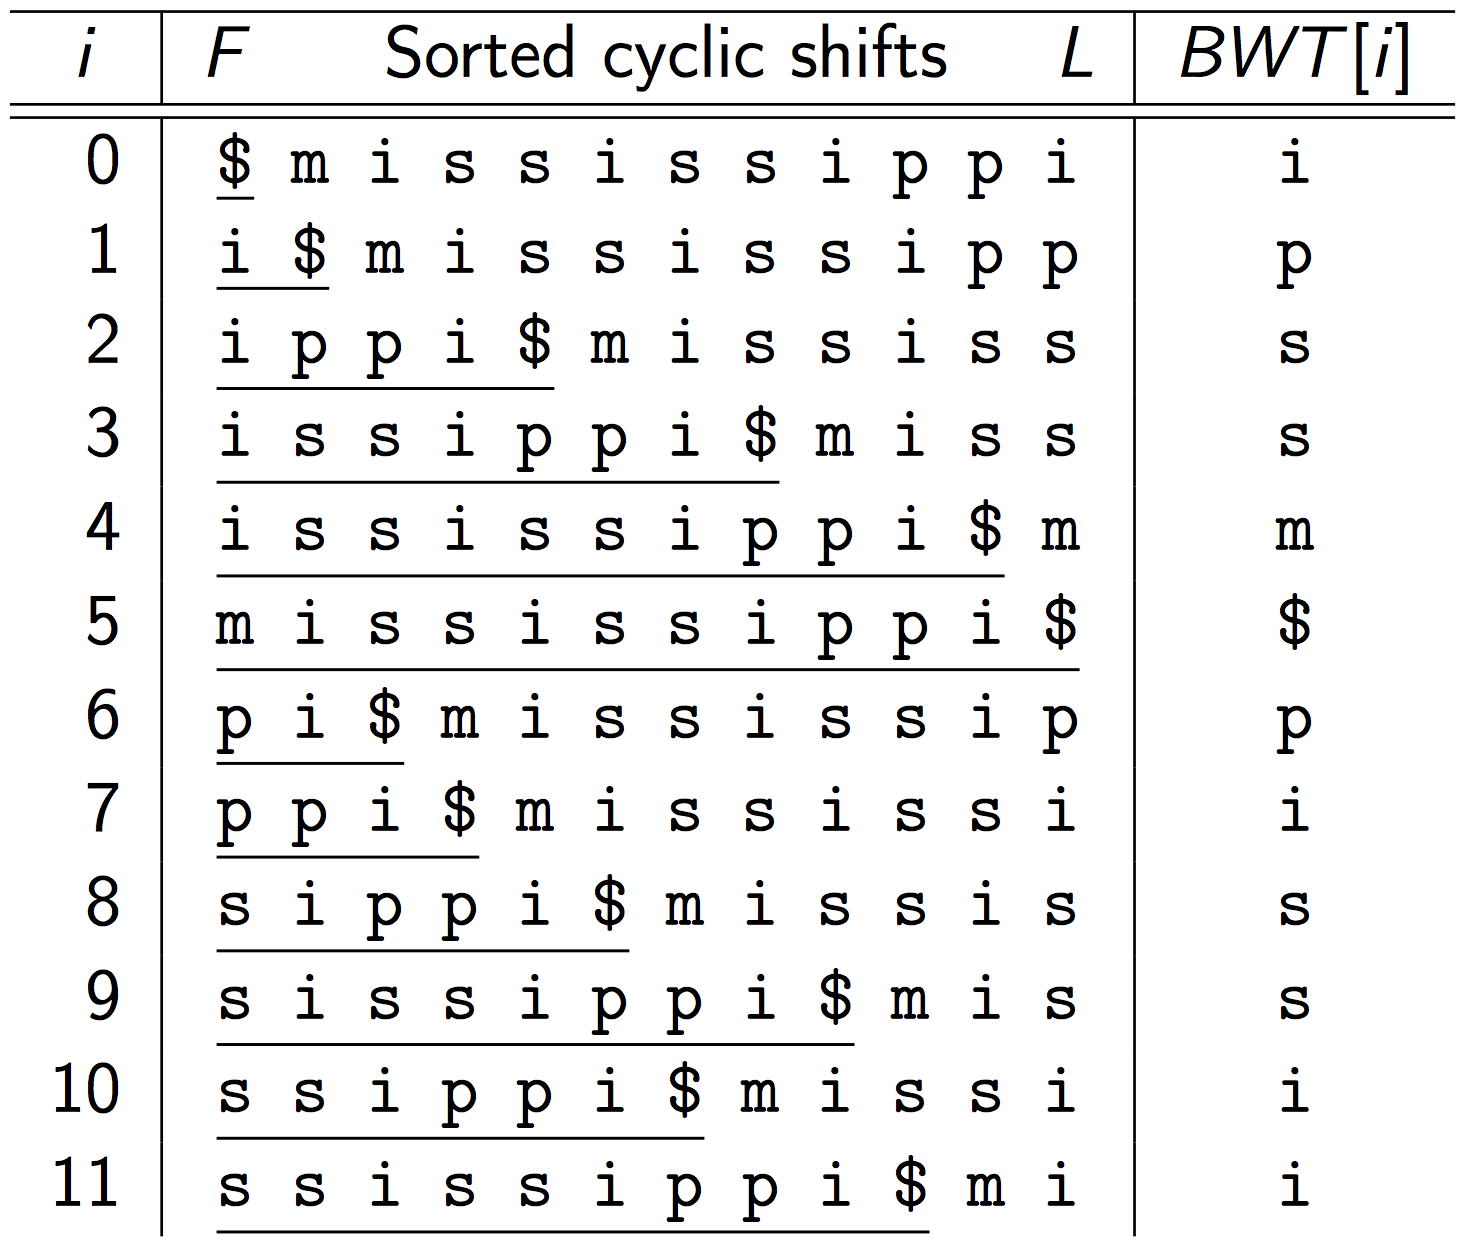
\includegraphics[scale=0.4]{Figure1.png}
\caption{BW Matrix}
\label{fig:bwm}
\end{center}
\end{figure}


The underlined sub sequences in $M$ are the suffixes of $T$. The character at $BWT[i]$ directly relates to the suffix array at $M[i]$. If a cyclic shift were performed on $M[i]$, $BWT[i]$ would be at the beginning of that row and the suffix would occur after $BWT[i]$. So, if $k$ is the position of $BWT[i]$ in $T$, then the suffix in $M[i]$ starts at position $k+1$ in $T$. Since $'\$'$ is the last character in the sequence, it is mapped to $0$. For Figure \ref{fig:bwm}, the following is the suffix array:

$$
SA = { 11, 10, 7, 4, 1, 0, 9, 8, 6, 3, 5, 2 }
$$

\newpage

The following algorithm uses a similar concept to reversing the $BWT$ to get $T$. However, instead it sets the $SA$ sequence.

\begin{algorithm}
\DontPrintSemicolon
\SetKwInOut{Input}{input}\SetKwInOut{Output}{output}
\SetKw{KwTo}{in}\SetKw{KwDownTo}{down to}
\Input{BWT of sequence T}
\Output{the suffix array SA[0..n-1]}
\BlankLine

$j \leftarrow 0$
\tcp*[h]{Indexer for BWT}\label{cmt}
\BlankLine
\For{$i$ \KwTo $n-2$ \KwDownTo $0$}{
  $SA[j] = i+1$ \;
  $j \leftarrow C\big(BWT[j]\big) + Rank_{BWT}(j, BWT[j]) - 1$
}

\caption{Create\_SA(BWT)}\label{algo_suffixArray}
\end{algorithm}

The performance of this algorithm largely depends on $C$ and $Rank_{BWT}$. $C$ can be implemented to have a time and space cost of $O(\sigma)$. $Rank_{BWT}$ could have a space cost of $O(nlog\sigma)$ and a time cost of $O(log\sigma)$, or a space cost of $O(n\cdot\sigma)$ and a time cost of $O(1)$. The former uses a wavelet tree, $W$, and the latter uses a letter frequency table, $LF$. 

The following is the $LF$ for the $BWT$:

\begin{figure}[h!]
\begin{center}
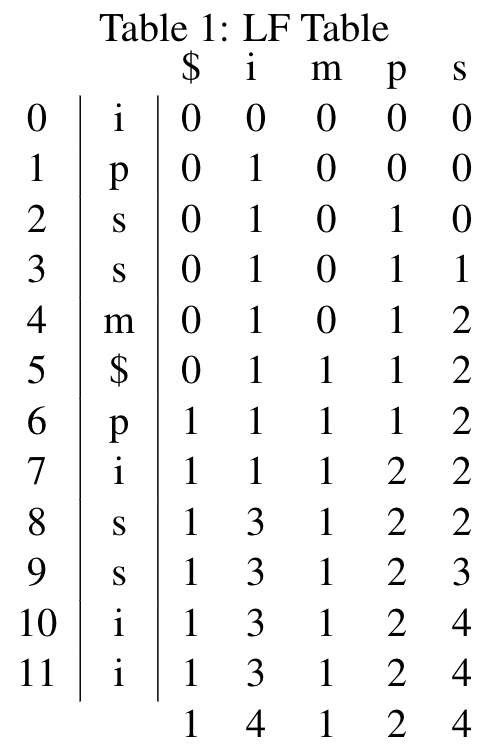
\includegraphics[scale=0.7]{Table1.png}
\label{fig:lf}
\end{center}
\end{figure}

The $jth$ column of $LF$ states that prior to this row, these are the number of occurrences of each letter in $\Sigma$. The pseudocode for $Rank_{BWT}$ using a letter frequency table would be as follows:

\newpage

\begin{algorithm}
\DontPrintSemicolon
\SetKwInOut{Input}{input}\SetKwInOut{Output}{output}
\SetKw{KwTo}{t}
\Input{i is current index in , c is character to rank}
\Output{r is the rank}
\BlankLine
\tcp{do i+1 to include the ith row}\label{cmt}
\Return{LF[i+1][c]}

\caption{Rank(i,c)}\label{algo_rank1}
\end{algorithm}

This proves that using $LF$ as a lookup table is constant time. The $Rank_{BWT}$ changes when using $W$:

\begin{algorithm}
\DontPrintSemicolon
\SetKwInOut{Input}{input}\SetKwInOut{Output}{output}
\SetKw{KwTo}{t}
\Input{i is current index in , c is character to rank}
\Output{r is the rank}
\BlankLine
$cur \leftarrow root$ \;
$r \leftarrow i$ \;
\While{$cur \neq leaf$}{
  $B \leftarrow cur.bit_vector$ \;
  \If{$B[r] == 0$}{
    $r \leftarrow rank_B(0,r)$ \;
    $cur \leftarrow cur.left_child$ \;
  }
  \Else{
    $r \leftarrow rank_B(1,r)$ \;
    $cur \leftarrow cur.right_child$ \;
  }
  $r \leftarrow r - 1$
}
\Return{r}

\caption{Rank(i,c)}\label{algo_rank2}
\end{algorithm}

Though the time cost of this method is $O(log\sigma)$, it is much slower than the $LF$ table because it is not constant time. The contant time that $LF$ provides does come with a cost. $LF$ has a space cost of $O(n\cdot\sigma)$, as can be seen in Figure 1. $W$ is much more space efficient. As can be seen in Figure 2, $W$ has a space cost of $O(nlog\sigma)$.

\begin{figure}[h!]
\begin{center}
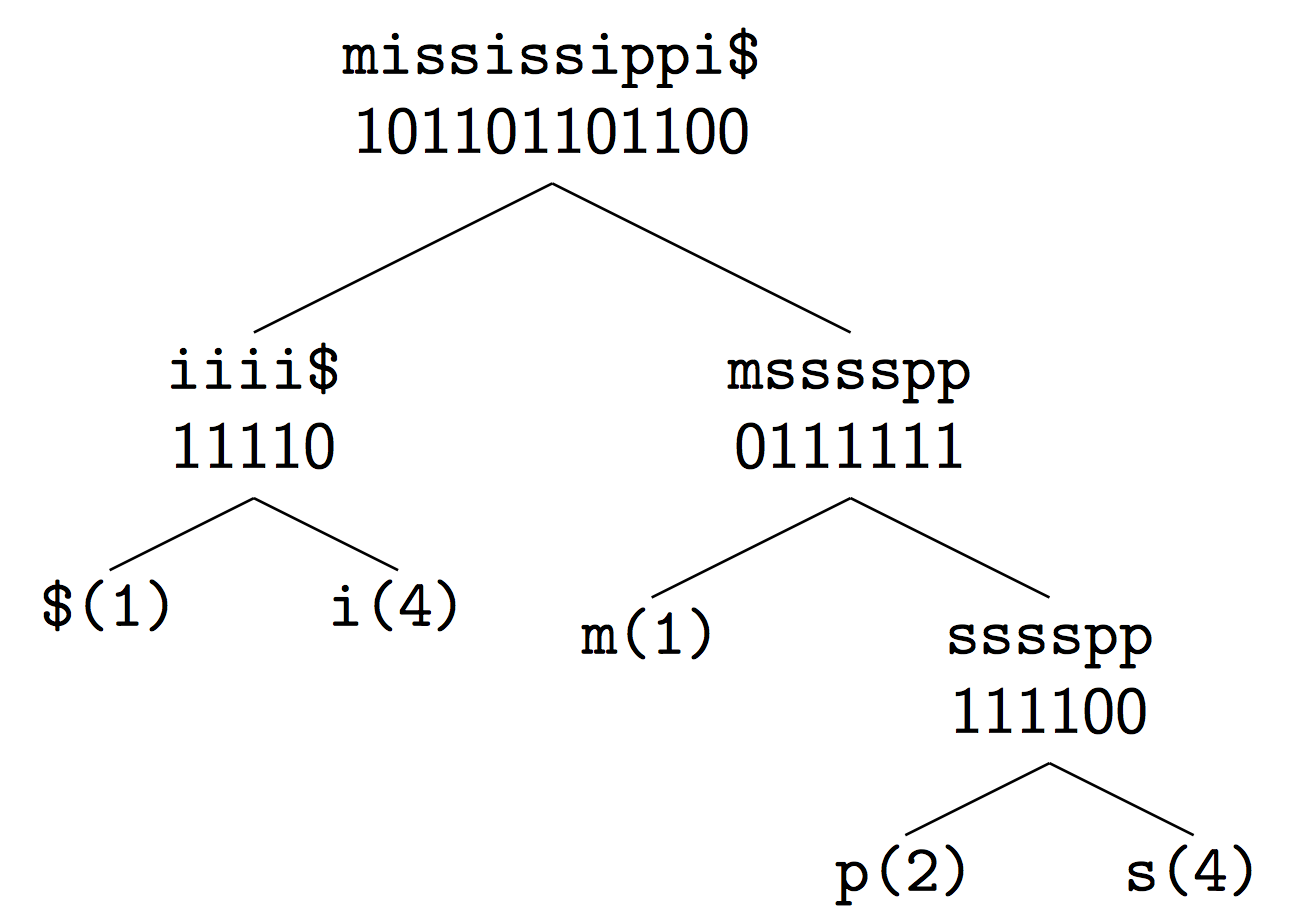
\includegraphics[scale=0.3]{Figure2.png}
\caption{Wavelet Tree of T}
\label{fig:wave}
\end{center}
\end{figure}

\newpage

$C$ can perform in $O(1)$, regardless if $W$ or $LF$ is used. It requires doing preprocessing of either the $W$ or $LF$. The leaf nodes in $W$ and the last row in $LF$. The preprocessing step would cost $O(\sigma)$ to create a lookup table of size $\sigma$. This lookup table at each position $c$, where $c$ is a character from $BWT$, would have a value that represents the number of characters that are less than $c$. The space cost for $C$ would be an additional $O(\sigma)$.

Given these two cases, Algorithm 1 can have different time and space costs. If memory usage needs to be conserved, using the wavelet tree will have a time cost of $O(nlog\sigma)$ and a space cost of $O(\sigma + nlog\sigma)$. If memory is not an issue, then using the letter frequency table will have a time cost of $O(n)$, which beats the wavelet tree. However, the space cost is $O(\sigma + n \cdot \sigma)$ which is far worse than the wavelet tree.

\end{document}




